\section{Technika sítí a protokolů - komunikační modely, způsob přenosu informace, základní struktura sítí, typy sítí, architektura komunikace systémů.}

\subsection{Komunikační modely}

Základním účelem komunikace je vzájemná výměna informací mezi dvěma uživateli (zdrojem a
spotřebičem). Lze ji rozdělit na dva typy komunikací: \textbf{komunikace uvnitř sítí} včetně dohledu nad touto komunikací, tj. určitá servisní část komunikace a~\textbf{komunikace mezi koncovými uživateli}, tj. komunikace nad sítěmi.

\subsubsection{Základní pojmy}

\textbf{Data} jsou reprezentace faktů, pojmů nebo instrukcí ve formalizované podobě vhodné pro
komunikaci, interpretace (výklad) informace pro strojové zpracování. \textbf{Informace} je význam, který mají data přiřazena, typicky pro uživatele.

Na obrázku \ref{q01_simplified_scheme_network} je mezi dvěma uživateli vyměňována informace nazvaná $m$. Informace $m$ je pomocí vstupního zařízení reprezentována jako data $g(t)$, ve formě časově proměnlivého signálu. V tomto okamžiku ještě není signál vhodný pro vysílání a musí být \enquote{přeložen} do podoby vhodné pro přenosové médium, tj. signálu $s(t)$, což je úkol vysílače. Tento signál je již přenášen médiem a na jeho druhé straně se objeví jako signál $r(t)$, který může být odlišný od původního signálu $s(t)$ následkem rušení či šumů v médiu. Signál $r(t)$ je konvertován v přijímači zpět do tvaru výstupních dat $g'(t)$, které mohou odpovídat vstupním datům přesně nebo přibližně. Nakonec je přes výstupní zařízení předána informace uživateli v podobě $m'$. Komunikací uvnitř sítě se rozumí část od vstupního k výstupnímu přenosovému zařízení, zatímco pro uživatele by se tato část měla jevit jako zcela transparentní.

\begin{figure}[ht]
	\centering
	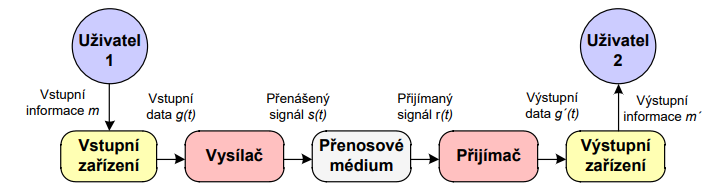
\includegraphics[width=\textwidth]{images/q01_simplified_scheme_network}
	\caption{Zjednodušené blokové schéma datovké komunikace}
	\label{q01_simplified_scheme_network}
\end{figure}

Komunikační sítě slouží vždy k tomu, aby pomocí nich mohli spolu komunikovat koncoví uživatelé, v
případě použití počítačů pak vzájemně komunikují odpovídající si (partnerské) procesy, které běží
každý na jednom z komunikujících počítačů (uvažujeme-li pouze komunikaci bod-bod). Základním
předpokladem pro komunikaci uživatelů je definice rozhraní mezi uživatelem a sítí. Rozhraní musí
definovat strukturu a formát předávaných uživatelských a řídicích dat.

\begin{figure}[ht]
	\centering
	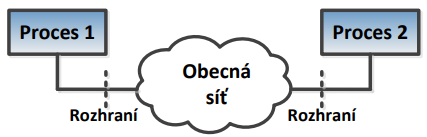
\includegraphics[width=\textwidth]{images/q01_simplified_scheme_processes}
	\caption{Zjednodušené blokové schéma komunikace mezi procesy pracujícími na~samostatných počítačích propojených obecnou sítí}
	\label{q01_simplified_scheme_processes}
\end{figure}

\clearpage
\section{Základní popis referenčního modelu ISO/OSI a srovnání s TCP/IP.}

\clearpage
\section{Základní popis síťového modelu TCP/IP a srovnání s ISO/OSI.}

\clearpage
\section{Principy komunikačních technik -- vícenásobné využití cest, zajištění obousměrné komunikace.}

\clearpage
\section{Fyzická vrstva přenosových systémů -- přenosová média, analogové a digitální modulace, klíčovací techniky, princip digitalizace řečového signálu.}

\clearpage
\section{Spojová vrstva přenosových systémů -- podvrstvy, rámce spojové vrstvy, adresace, metody zajištění spolehlivého přenosu.}

\clearpage
\section{Síťová vrstva přenosových systémů -- spínání paketů, služby síťové vrstvy, IPv4 adresy, techniky směrování, IPv4 datagram.}

\clearpage
\section{Síťová vrstva přenosových systémů -- tunelování paketů, ARP, NAT, ICMPv4, IPv6.}

\clearpage
\section{Transportní vrstva přenosových systémů -- služby transportní vrstvy, UDP protokol, TCP protokol.}

\clearpage
\section{Aplikační vrstva přenosových systémů -- DHCP protokol, DNS systém, přenos souborů, webové protokoly, elektronická pošta.}
